%package list
\documentclass{article}
\usepackage[top=3cm, bottom=3cm, outer=3cm, inner=3cm]{geometry}
\usepackage{multicol}
\usepackage{graphicx}
\usepackage{url}
%\usepackage{cite}
\usepackage{hyperref}
\usepackage{array}
%\usepackage{multicol}
\newcolumntype{x}[1]{>{\centering\arraybackslash\hspace{0pt}}p{#1}}
\usepackage{natbib}
\usepackage{pdfpages}
\usepackage{multirow}
\usepackage[normalem]{ulem}
\useunder{\uline}{\ul}{}
\usepackage{svg}
\usepackage{xcolor}
\usepackage{listings}
\lstdefinestyle{ascii-tree}{
    literate={├}{|}1 {─}{--}1 {└}{+}1 
  }
\lstset{basicstyle=\ttfamily,
  showstringspaces=false,
  commentstyle=\color{red},
  keywordstyle=\color{blue}
}
%\usepackage{booktabs}
\usepackage{caption}
\usepackage{subcaption}
\usepackage{float}
\usepackage{array}

\newcolumntype{M}[1]{>{\centering\arraybackslash}m{#1}}
\newcolumntype{N}{@{}m{0pt}@{}}


%%%%%%%%%%%%%%%%%%%%%%%%%%%%%%%%%%%%%%%%%%%%%%%%%%%%%%%%%%%%%%%%%%%%%%%%%%%%
%%%%%%%%%%%%%%%%%%%%%%%%%%%%%%%%%%%%%%%%%%%%%%%%%%%%%%%%%%%%%%%%%%%%%%%%%%%%
\newcommand{\itemStudent}{Diego Renato Llerena Tellez Mauricio Zegarra Puma  Andre David Delgado Allpan Gonzalo Rail Layme Mamani Andre Hilacondo Begazo @unsa.edu.pe}
\newcommand{\itemCourse}{Estructura de datos y algoritmos}
\newcommand{\itemUniversity}{Universidad Nacional de San Agustín de Arequipa}
\newcommand{\itemFaculty}{Facultad de Ingeniería de Producción y Servicios}
\newcommand{\itemDepartment}{Departamento Académico de Ingeniería de Sistemas e Informática}
\newcommand{\itemSchool}{Escuela Profesional de Ingeniería de Sistemas}
\newcommand{\itemAcademic}{2023 - A}
\newcommand{\itemInput}{Del 21 Junio 2023}
\newcommand{\itemOutput}{Al 28 Junio 2023}
\newcommand{\itemPracticeNumber}{05}
\newcommand{\itemTheme}{Arboles AVL}
%%%%%%%%%%%%%%%%%%%%%%%%%%%%%%%%%%%%%%%%%%%%%%%%%%%%%%%%%%%%%%%%%%%%%%%%%%%%
%%%%%%%%%%%%%%%%%%%%%%%%%%%%%%%%%%%%%%%%%%%%%%%%%%%%%%%%%%%%%%%%%%%%%%%%%%%%

\usepackage[english,spanish]{babel}
\usepackage[utf8]{inputenc}
\AtBeginDocument{\selectlanguage{spanish}}
\renewcommand{\figurename}{Figura}
\renewcommand{\refname}{Referencias}
\renewcommand{\tablename}{Tabla} %esto no funciona cuando se usa babel
\AtBeginDocument{%
	\renewcommand\tablename{Tabla}
}

\usepackage{fancyhdr}
\pagestyle{fancy}
\fancyhf{}
\setlength{\headheight}{30pt}
\renewcommand{\headrulewidth}{1pt}
\renewcommand{\footrulewidth}{1pt}
\fancyhead[L]{\raisebox{-0.2\height}{
\includegraphics[width=3cm]{img/logo_episunsa.png}}}
\fancyhead[C]{\fontsize{7}{7}\selectfont	\itemUniversity \\ \itemFaculty \\ \itemDepartment \\ \itemSchool \\ \textbf{\itemCourse}}
\fancyhead[R]{\raisebox{-0.2\height}{
\includegraphics[width=1.2cm]{img/logo_abet}}}
\fancyfoot[L]{Estudiante Diego Llerena Tellez}
\fancyfoot[C]{\itemCourse}
\fancyfoot[R]{Página \thepage}

% para el codigo fuente
\usepackage{listings}
\usepackage{color, colortbl}
\definecolor{dkgreen}{rgb}{0,0.6,0}
\definecolor{gray}{rgb}{0.5,0.5,0.5}
\definecolor{mauve}{rgb}{0.58,0,0.82}
\definecolor{codebackground}{rgb}{0.95, 0.95, 0.92}
\definecolor{tablebackground}{rgb}{0.8, 0, 0}

\lstset{frame=tb,
	language=bash,
	aboveskip=3mm,
	belowskip=3mm,
	showstringspaces=false,
	columns=flexible,
	basicstyle={\small\ttfamily},
	numbers=none,
	numberstyle=\tiny\color{gray},
	keywordstyle=\color{blue},
	commentstyle=\color{dkgreen},
	stringstyle=\color{mauve},
	breaklines=true,
	breakatwhitespace=true,
	tabsize=3,
	backgroundcolor= \color{codebackground},
}

\begin{document}
	
	\vspace*{10px}
	
	\begin{center}	
		\fontsize{17}{17} \textbf{ Informe de Laboratorio \itemPracticeNumber}
	\end{center}
	\centerline{\textbf{\Large Tema: \itemTheme}}
	%\vspace*{0.5cm}	

	\begin{flushright}
		\begin{tabular}{|M{2.5cm}|N|}
			\hline 
			\rowcolor{tablebackground}
			\color{white} \textbf{Nota}  \\
			\hline 
			     \\[30pt]
			\hline 			
		\end{tabular}
	\end{flushright}	

	\begin{table}[H]
		\begin{tabular}{|x{4.7cm}|x{4.8cm}|x{4.8cm}|}
			\hline 
			\rowcolor{tablebackground}
			\color{white} \textbf{Estudiante} & \color{white}\textbf{Escuela}  & \color{white}\textbf{Asignatura}   \\
			\hline 
			{\itemStudent \par} & \itemSchool & {\itemCourse \par}     \\
			\hline 			
		\end{tabular}
	\end{table}		
	
	\begin{table}[H]
		\begin{tabular}{|x{4.7cm}|x{4.8cm}|x{4.8cm}|}
			\hline 
			\rowcolor{tablebackground}
			\color{white}\textbf{Laboratorio} & \color{white}\textbf{Tema}  & \color{white}\textbf{Duración}   \\
			\hline 
			\itemPracticeNumber & \itemTheme & 02 horas   \\
			\hline 
		\end{tabular}
	\end{table}
	
	\begin{table}[H]
		\begin{tabular}{|x{4.7cm}|x{4.8cm}|x{4.8cm}|}
			\hline 
			\rowcolor{tablebackground}
			\color{white}\textbf{Semestre académico} & \color{white}\textbf{Fecha de inicio}  & \color{white}\textbf{Fecha de entrega}   \\
			\hline 
			\itemAcademic & \itemInput &  \itemOutput  \\
			\hline 
		\end{tabular}
	\end{table}
	
	\section{Tarea}
	\begin{itemize}		
		\item Elabore un informe implementando Arboles AVL con toda la lista de operaciones search(),getMin(), getMax(), parent(), son(), insert(), remove(). 
		\item INPUT: Una sola palabra en mayúsculas.
		\item OUTPUT: Se debe contruir el árbol AVL considerando el valor decimal de su código ascii.
		\item Luego, pruebe todas sus operaciones implementadas.
		\item Estudie la libreria Graph Stream para obtener una salida gráfica de su implementación.
		\item
Utilice todas las recomendaciones dadas por el docente
	\end{itemize}
		
	\section{Equipos, materiales y temas utilizados}
	\begin{itemize}
		\item Sistema Operativo (GNU/Linux de preferencia).
		\item GNU Vim.
		\item Git.
		\item Cuenta en GitHub con el correo institucional.
	\end{itemize}
	
	\section{URL de Repositorio Github}
	\begin{itemize}
		\item URL del Repositorio GitHub para clonar o recuperar.
		\item \url{https://github.com/MauricioZegarra/Laboratorio_05_EDA.git}
	\end{itemize}
	
	\section{Actividad realizada}
	
	\subsection{Clase Nodo y Clase AVL}
	\begin{itemize}	
		\item Para la realización de este laboratorio se nos pidio implementar los métodos de un Árbol AVL y mostar su funcionalidad. Un árbol AVL es un tipo especial de árbol de búsqueda binario que trata de estar lo más balanceado posible, es decir que la diferencia entre el sub-arbol derecho e izquierdo debe de ser igual a 0 o deber -1 o 1. A continuación se muestra el código generado para la resolución de los ejercicios.
		\item Primero se crea la clase Nodo que es la base para la implementación de las listas enlazadas.
	\end{itemize}	
		
	\begin{lstlisting}[language=bash,caption={Creando la Clase Nodo}][H]
		public class Nodo<E> {

    private E data;
    private Nodo<E> left;
    private Nodo<E> right;
    private int bf;

    public Nodo(E data, Nodo<E> left, Nodo<E> right) {
        this.data = data;
        this.left = left;
        this.right = right;
        this.bf = 0;
    }

    public int getBf() {
        return bf;
    }

    public void setBf(int bf) {
        this.bf = bf;
    }

    public Nodo(E data) {
        this(data, null, null);
    }

    public E getData() {
        return this.data;
    }

    public void setData(E data) {
        this.data = data;
    }

    public Nodo<E> getLeft() {
        return this.left;
    }

    public void setLeft(Nodo<E> left) {
        this.left = left;
    }

    public Nodo<E> getRight() {
        return this.right;
    }

    public void setRight(Nodo<E> right) {
        this.right = right;
    }

    public String toString() {
        return this.data.toString() + "(" + this.bf + ")";
    }
}
	\end{lstlisting}
	\begin{itemize}	
		\item El código implementa una estructura de datos conocida como Arbol AVL.
		\item La clase AVL es el contenedor principal que representa el Arbol AVL. 			\item Está parametrizada con el tipo T, que debe ser un tipo comparable.
		\item La clase Nodo representa los nodos individuales del Arbol AVL. Cada nodo contiene un dato de tipo T, referencias al nodo izquierdo y derecho, y un campo para almacenar la altura del nodo 
	\end{itemize}
	\begin{lstlisting}[language=bash,caption={Clase AVL: Base}][H]
	public class Avl<E extends Comparable<E>> {
    		private Nodo<E> root;
    		private boolean height;

    public Avl() {
        this.root = null;
    }

    public boolean isEmpty() {
        return this.root == null;
    }
	\end{lstlisting}	
	\begin{itemize}
	\item \texttt{public void insert(T input) throws ExceptionNoFound { ... }} - Inserta un elemento en el árbol AVL.
\item \texttt{private Node<T> rotateRSR(Node<T> xNode) { ... }} - Realiza una rotación hacia la derecha en el árbol AVL.
\item \texttt{private Node<T> rotateRSL(Node<T> yNode) { ... }} - Realiza una rotación hacia la izquierda en el árbol AVL.
	\end{itemize}
	\begin{lstlisting}[language=bash,caption={Clase AVL: Metodos de rotación derecha e izquierda}][H]   
	private Nodo<E> rotateRSR(Nodo<E> node) {
        Nodo<E> son = node.getLeft();
        node.setLeft(son.getRight());
        son.setRight(node);
        node = son;
        return node;
    }

    private Nodo<E> rotateRSL(Nodo<E> node) {
        Nodo<E> son = node.getRight();
        node.setRight(son.getLeft());
        son.setLeft(node);
        node = son;
        return node;
    }
	\end{lstlisting}	
	
	\begin{lstlisting}[language=bash,caption={Clase AVL:Metodo de balance a la Derecha }][H]
	private Nodo<E> balanceToRight(Nodo<E> node) {
        Nodo<E> son = node.getLeft();
        if (son.getBf() == -1) {
            node.setBf(0);
            son.setBf(0);
            node = rotateRSR(node);
        } else if (son.getBf() == 1) {
            Nodo<E> gSon = son.getRight();
            switch (gSon.getBf()) {
                case 1:
                    node.setBf(0);
                    son.setBf(1);
                    break;
                case 0:
                    node.setBf(0);
                    son.setBf(0);
                    break;
                case -1:
                    node.setBf(-1);
                    son.setBf(0);
                    break;
            }
            gSon.setBf(0);

            node.setLeft(rotateRSL(son));
            node = rotateRSR(node);
        }
        return node;
    }
	\end{lstlisting}	
	\begin{lstlisting}[language=bash,caption={Clase AVL: Método de balance a la izquierda}][H]
		private Nodo<E> balanceToLeft(Nodo<E> node) {
        Nodo<E> son = node.getRight();
        if (son.getBf() == 1) {
            node.setBf(0);
            son.setBf(0);
            node = rotateRSL(node);
        } else if (son.getBf() == -1) {
            Nodo<E> gSon = son.getLeft();
            switch (gSon.getBf()) {
                case -1:
                    node.setBf(0);
                    son.setBf(-1);
                    break;
                case 0:
                    node.setBf(0);
                    son.setBf(0);
                    break;
                case 1:
                    node.setBf(1);
                    son.setBf(0);
                    break;
            }
            gSon.setBf(0);

            node.setRight(rotateRSR(son));
            node = rotateRSL(node);
        }
        return node;
    }
	\end{lstlisting}
	
	\begin{lstlisting}[language=bash,caption={Clase AVL: Método Search()}][H]
		public E search(E x) throws ExceptionNoFound {
        Nodo<E> aux = search(x, this.root);
        if (aux == null) {
            throw new ExceptionNoFound("Elemento no se encuentra en el arbol");
        }
        return aux.getData();
    }
    
    		private Nodo<E> search(E x, Nodo<E> current) throws ExceptionNoFound {
        if (current == null) {
            return null;
        } else {
            int resC = current.getData().compareTo(x);
            if (resC == 0) {
                return current;
            }
            if (resC < 0) {
                return search(x, current.getRight());
            } else {
                return search(x, current.getLeft());
            }
        }
    }
	\end{lstlisting}
	
	\begin{lstlisting}[language=bash,caption={Clase AVL: Método getMax()}][H]
		public E getMax() throws ExceptionNoFound {
        if (isEmpty()) {
            throw new ExceptionNoFound("El arbol esta vacio");
        }

        Nodo<E> maxNode = getMaxNode(root);
        return maxNode.getData();
    }

    private Nodo<E> getMaxNode(Nodo<E> current) {
        if (current.getRight() == null) {
            return current;
        }
        return getMaxNode(current.getRight());
    }
	\end{lstlisting}
	
	\begin{lstlisting}[language=bash,caption={Clase AVL: Método getMin()}][H]
		public E getMin() throws ExceptionNoFound {
        if (isEmpty()) {
            throw new ExceptionNoFound("El arbol esta vacio");
        }

        Nodo<E> minNode = getMinNode(root);
        return minNode.getData();
    }

    private Nodo<E> getMinNode(Nodo<E> current) {
        if (current.getLeft() == null) {
            return current;
        }
        return getMinNode(current.getLeft());
    }
	\end{lstlisting}
	\begin{lstlisting}[language=bash,caption={Clase AVL: Método getMin()}][H]
		public E getMin() throws ExceptionNoFound {
        if (isEmpty()) {
            throw new ExceptionNoFound("El arbol esta vacio");
        }

        Nodo<E> minNode = getMinNode(root);
        return minNode.getData();
    }

    private Nodo<E> getMinNode(Nodo<E> current) {
        if (current.getLeft() == null) {
            return current;
        }
        return getMinNode(current.getLeft());
    }
	\end{lstlisting}
	
	\begin{lstlisting}[language=bash,caption={Clase AVL: Método son()}][H]
	//  son busca si ambos elementos estan presentes y  si a es padre de b, 
    //de lo contrario, devuelve false. 
    public boolean son(E a, E b) throws ExceptionNoFound {
        return son(a, b, this.root);
    }

    private boolean son(E a, E b, Nodo<E> current) throws ExceptionNoFound {
        if (current == null) {
            return false;
        }

        boolean aEncontrado = false;
        boolean bEncontrado = false;

        if (current.getData().equals(a)) {
            aEncontrado = true;
        } else if (current.getData().equals(b)) {
            bEncontrado = true;
        }

        if (aEncontrado && bEncontrado) {
            return true;
        }

        boolean hijoEnIzquierda = son(a, b, current.getLeft());
        boolean hijoEnDerecha = son(a, b, current.getRight());

        if (aEncontrado || bEncontrado || hijoEnIzquierda || hijoEnDerecha) {
            return true;
        }

        return false;
    }
	\end{lstlisting}
	\begin{lstlisting}[language=bash,caption={Clase AVL: Método parent()}][H]
	//metodo parent busca el padre mas cercano entre dos nodos
    public E parent(E a, E b) throws ExceptionNoFound {
    return parent(a, b, this.root);
    }

    private E parent(E a, E b, Nodo<E> current) throws ExceptionNoFound {
        if (current == null) {
            throw new ExceptionNoFound("Elemento no se encuentra en el arbol");
        }

        if ((current.getLeft() != null && current.getLeft().getData().equals(a) && current.getRight() != null && current.getRight().getData().equals(b))
                || (current.getRight() != null && current.getRight().getData().equals(a) && current.getLeft() != null && current.getLeft().getData().equals(b))) {
            return current.getData();
        }

        E parentEnIzquierda = parent(a, b, current.getLeft());
        E parentEnDerecha = parent(a, b, current.getRight());

        if (parentEnIzquierda != null) {
            return parentEnIzquierda;
        } else if (parentEnDerecha != null) {
            return parentEnDerecha;
        }

        return null;
    }
	\end{lstlisting}
		
	\subsection{Clase GraphAVLWord.java}
	\begin{itemize}
        	\item Esta clase se genera graficamente el árbol de busqueda binaria.
\item Establece la propiedad del sistema "org.graphstream.ui" en "swing" para utilizar la interfaz de usuario de Swing para mostrar el grafo.
	\item Crea un objeto Graph llamado graph utilizando la implementación SingleGraph.
\end{itemize}
	
	\begin{lstlisting}[language=bash,caption={Clase GraphAVLWord: Main}][H]
	public static void main(String[] args) throws ExceptionNoFound {

        System.setProperty("org.graphstream.ui", "swing");

        Scanner sc = new Scanner(System.in);
        
        System.out.print("Introduzca la palabra: ");
        String word = sc.next();
        
        Avl<Character> avl = new Avl<Character>();
        
        for (int i = 0; i < word.length(); i++) {
            avl.insert(word.charAt(i));
        }
        
        System.out.println("\nLa cabeza del AVL es: " + avl.getRoot());

        GraphAVLWord<Character> graphPrinter = new GraphAVLWord<Character>(avl);
        graphPrinter.print();
    }

    public void print() {
        addNodes(this.avl.getRoot(), null);
        addEdges(this.avl.getRoot());
        
        this.graph.display();
    }
	\end{lstlisting}
	\begin{lstlisting}[language=bash,caption={Clase GraphAVLWord: addNodes()}][H]
	private void addNodes(Nodo<E> node, Node parentNode) {
        if (node != null) {
            Node graphNode = this.graph.addNode(node.getData().toString());
            graphNode.setAttribute("ui.label", node.getData().toString());
            if (parentNode != null) {
                this.graph.addEdge(parentNode.getId() + "_" + graphNode.getId(), parentNode, graphNode);
            }
            addNodes(node.getLeft(), graphNode);
            addNodes(node.getRight(), graphNode);
        }
    }
	\end{lstlisting}
	\begin{lstlisting}[language=bash,caption={Clase GraphAVLWord: addEdges()}][H]
	private void addEdges(Nodo<E> current) {
        if (current.getLeft() != null) {
            String edgeId = current.getData().toString() + "_" + current.getLeft().getData().toString();
            if (this.graph.getEdge(edgeId) == null) {
                this.graph.addEdge(edgeId, current.getData().toString(), current.getLeft().getData().toString());
            }
            addEdges(current.getLeft());
        }

        if (current.getRight() != null) {
            String edgeId = current.getData().toString() + "_" + current.getRight().getData().toString();
            if (this.graph.getEdge(edgeId) == null) {
                this.graph.addEdge(edgeId, current.getData().toString(), current.getRight().getData().toString());
            }
            addEdges(current.getRight());
        }
    }
	\end{lstlisting}
	\subsection{Ejecuciones}
	\begin{itemize}	
		\item Ejecución del árbol con los nombres Diego y Andre
	\end{itemize}
	\begin{figure}[H]
	\centering
	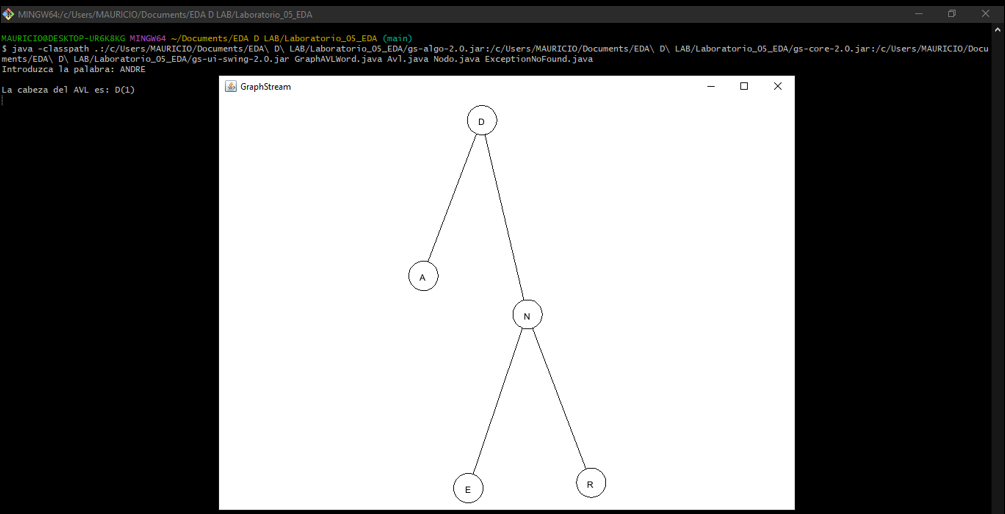
\includegraphics[width=0.7\textwidth,keepaspectratio]{img/ejecucion_word_ANDRE.png}
	\caption{ejecuciones: ejecucion de la clase Aplicacion con "ANDRE"}
\end{figure}
\begin{figure}[H]
	\centering
	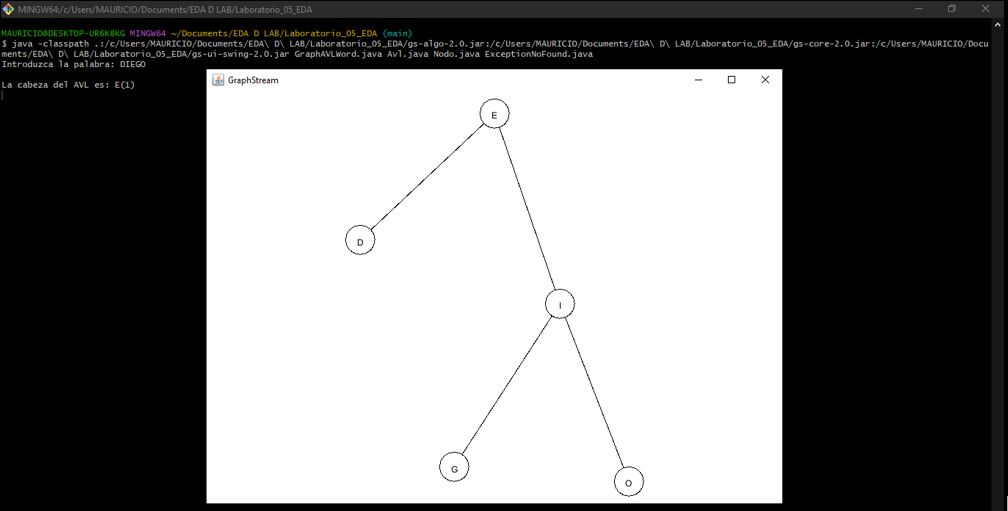
\includegraphics[width=0.7\textwidth,keepaspectratio]{img/ejecucion_word_DIEGO.png}
	\caption{ejecuciones: ejecucion de la clase Aplicacion con "DIEGO"}
\end{figure}

	\subsection{Estructura de laboratorio 05}
	\begin{itemize}	
		\item El contenido que se entrega en este laboratorio es el siguiente:
	\end{itemize}
	
\begin{lstlisting}[style=ascii-tree]
Laboratorio_05_EDA/
|---Avl.java
|---ExceptionNoFound.java
|---GraphAVLWord.java
|---Nodo.java
|---gs-algo-2.0.jar
|---gs-core-2.0.jar
|---gs-ui-swing-2.0.jar
|--- latex
    |--- img
    |   |--- logo_abet.png
    |   |--- logo_episunsa.png
    |   |--- logo_unsa.jpg
    |   |--- ejecucion_word_ANDRE.jpg
    |   |--- ejecucion_word_DIEGO.jpg
    |   |--- Pas.png  
    |--- Lab05 Arboles AVL.pdf    
    |--- Lab05 Arboles AVL.tex
\end{lstlisting}    

\section{Pregunta:}
	\begin{itemize}
		\item ¿Explique como es el algoritmo que implementó para obtener el factor de equilibrio de un nodo?
	\item El factor de equilibrio (bf) se basa en la diferencia de alturas entre subárbol izquierdo y el subárbol derecho del nodo. Este se utiliza para determinar si un nodo está balanceado o si se requieren rotaciones para mantener balanceado el árbol.

Sobre el algoritmo que implementamos (`insert` y `remove`), primero se realiza un recorrido hasta llegar al nodo afectado (en el bf), después se calcula la diferencia de alturas, esta diferencia se almacena en `bf` del nodo.

Ahora, dependiendo del valor se realiza la acción siguiente:

- Si el factor de balance es -1, 0 o 1, el nodo se considera balanceado y no se requieren ajustes.
- Si el factor de balance es -2 o 2, indica que el nodo está desbalanceado y se requieren rotaciones y ajustes para restaurar el balance.
- En el caso de una inserción, si el factor de balance es 2, se llama al método `balanceToLeft` para realizar rotaciones y ajustes hacia la izquierda.
- En el caso de una eliminación, si el factor de balance es -2, se llama al método `balanceToRight` para realizar rotaciones y ajustes hacia la derecha.
\end{itemize}


	\section{\textcolor{red}{Rúbricas}}
	
	\subsection{\textcolor{red}{Entregable Informe}}
	\begin{table}[H]
		\caption{Tipo de Informe}
		\setlength{\tabcolsep}{0.5em} % for the horizontal padding
		{\renewcommand{\arraystretch}{1.5}% for the vertical padding
		\begin{tabular}{|p{3cm}|p{12cm}|}
			\hline
			\multicolumn{2}{|c|}{\textbf{\textcolor{red}{Informe}}}  \\
			\hline 
			\textbf{\textcolor{red}{Latex}} & \textcolor{blue}{El informe está en formato PDF desde Latex,  con un formato limpio (buena presentación) y facil de leer.}   \\ 
			\hline 
			
			
		\end{tabular}
	}
	\end{table}
	
	\clearpage
	
	\subsection{\textcolor{red}{Rúbrica para el contenido del Informe y demostración}}
	\begin{itemize}			
		\item El alumno debe marcar o dejar en blanco en celdas de la columna \textbf{Checklist} si cumplio con el ítem correspondiente.
		\item Si un alumno supera la fecha de entrega,  su calificación será sobre la nota mínima aprobada, siempre y cuando cumpla con todos lo items.
		\item El alumno debe autocalificarse en la columna \textbf{Estudiante} de acuerdo a la siguiente tabla:
	
		\begin{table}[ht]
			\caption{Niveles de desempeño}
			\begin{center}
			\begin{tabular}{ccccc}
    			\hline
    			 & \multicolumn{4}{c}{Nivel}\\
    			\cline{1-5}
    			\textbf{Puntos} & Insatisfactorio 25\%& En Proceso 50\% & Satisfactorio 75\% & Sobresaliente 100\%\\
    			\textbf{2.0}&0.5&1.0&1.5&2.0\\
    			\textbf{4.0}&1.0&2.0&3.0&4.0\\
    		\hline
			\end{tabular}
		\end{center}
	\end{table}	
	
	\end{itemize}
	
	\begin{table}[H]
		\caption{Rúbrica para contenido del Informe y demostración}
		\setlength{\tabcolsep}{0.5em} % for the horizontal padding
		{\renewcommand{\arraystretch}{1.5}% for the vertical padding
		%\begin{center}
		\begin{tabular}{|p{2.7cm}|p{7cm}|x{1.3cm}|p{1.2cm}|p{1.5cm}|p{1.1cm}|}
			\hline
    		\multicolumn{2}{|c|}{Contenido y demostración} & Puntos & Checklist & Estudiante & Profesor\\
			\hline
			\textbf{1. GitHub} & Hay enlace URL activo del directorio para el  laboratorio hacia su repositorio GitHub con código fuente terminado y fácil de revisar. &2 &X &2 & \\ 
			\hline
			\textbf{2. Commits} &  Hay capturas de pantalla de los commits más importantes con sus explicaciones detalladas. (El profesor puede preguntar para refrendar calificación). &4 &X &4 & \\ 
			\hline 
			\textbf{3. Código fuente} &  Hay porciones de código fuente importantes con numeración y explicaciones detalladas de sus funciones. &2 &X &2 & \\ 
			\hline 
			\textbf{4. Ejecución} & Se incluyen ejecuciones/pruebas del código fuente  explicadas gradualmente. &2 &X &2 & \\ 
			\hline			
			\textbf{5. Pregunta} & Se responde con completitud a la pregunta formulada en la tarea.  (El profesor puede preguntar para refrendar calificación).  &2 &X &2 & \\ 
			\hline	
			\textbf{6. Fechas} & Las fechas de modificación del código fuente estan dentro de los plazos de fecha de entrega establecidos. &2 &X &1 & \\ 
			\hline 
			\textbf{7. Ortografía} & El documento no muestra errores ortográficos. &2 &X &2 & \\ 
			\hline 
			\textbf{8. Madurez} & El Informe muestra de manera general una evolución de la madurez del código fuente,  explicaciones puntuales pero precisas y un acabado impecable.   (El profesor puede preguntar para refrendar calificación).  &4 &X &4 & \\ 
			\hline
			\multicolumn{2}{|c|}{\textbf{Total}} &20 & &19 & \\ 
			\hline
		\end{tabular}
		%\end{center}
		%\label{tab:multicol}
		}
	\end{table}
	
\clearpage

\section{Referencias}
\begin{itemize}			
	\item \url{https://www.geeksforgeeks.org/introduction-to-avl-tree/}
	\item \url{https://www.geeksforgeeks.org/insertion-in-an-avl-tree/}
	\item \url{https://www.geeksforgeeks.org/deletion-in-an-avl-tree/}
	\item \url{https://www.javatpoint.com/avl-tree}
	\item \url{https://docs.oracle.com/javase/tutorial/java/generics/types.html}
	\item \url{https://algorithmtutor.com/Data-Structures/Tree/AVL-Trees/}
\end{itemize}	
	
%\clearpage
%\bibliographystyle{apalike}
%\bibliographystyle{IEEEtranN}
%\bibliography{bibliography}
			
\end{document}